% Fidelity vs. perceptual quality of every baseline at native resolution (DPDD, 76 test scenes, 6720x4480).
% Data: handoff/from_secure/2026-10-05_h3.md (native, x4 + HAT-L / SwinIR-real / Real-HAT / OSEDiff, DATSR),
% 2026-10-06_h4.md (bicubic, S3Diff, VOSR; identical where re-run), fusion rows 2026-10-04_h2.md (tuned on val).
% Columns: PSNR (dB) and DISTS on the whole native image. x4 rows: DRBNet (D) or Bokehlicious (B) anchor.
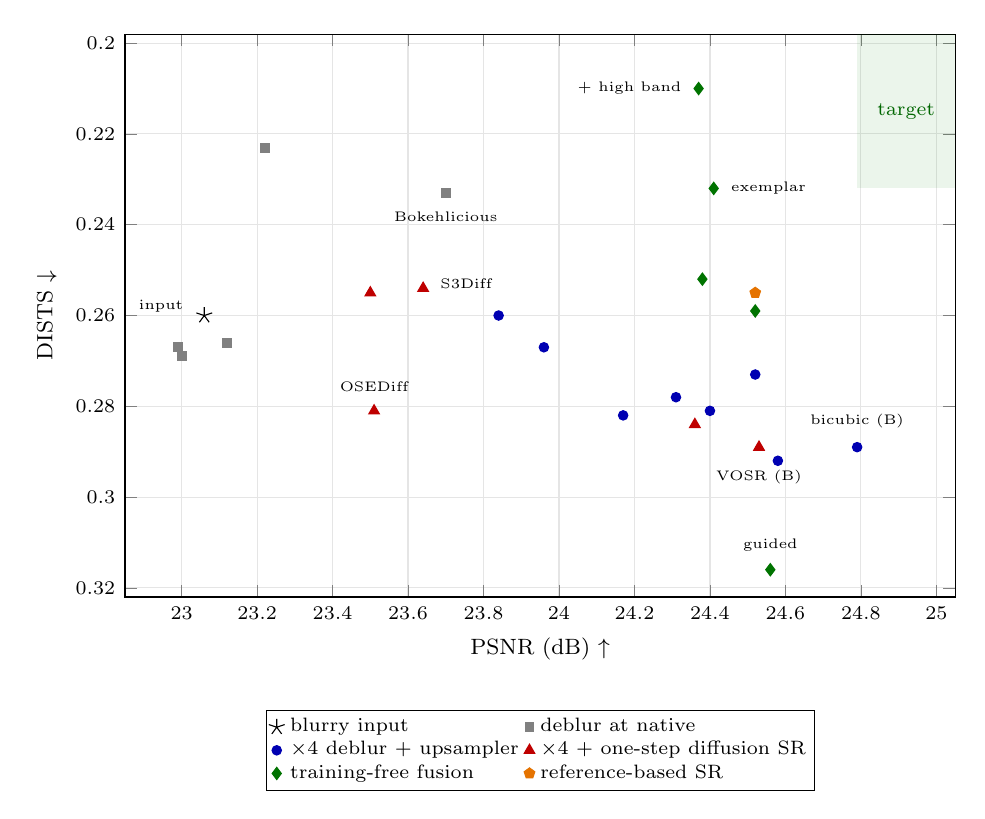
\begin{tikzpicture}
\begin{axis}[
  width=\linewidth, height=0.72\linewidth,
  xlabel={PSNR (dB) $\uparrow$}, ylabel={DISTS $\downarrow$},
  y dir=reverse, xmin=22.85, xmax=25.05, ymin=0.198, ymax=0.322,
  tick label style={font=\scriptsize}, label style={font=\footnotesize},
  legend style={font=\scriptsize, at={(0.5,-0.2)}, anchor=north, legend columns=2, row sep=-2pt, inner sep=1pt},
  legend cell align=left, grid=major, grid style={gray!20},
]
% target region: fidelity of the best low-resolution pipeline with the texture of the exemplar transfer
\fill[green!50!black, opacity=0.08] (axis cs:24.79,0.198) rectangle (axis cs:25.05,0.232);
\node[font=\scriptsize, text=green!40!black, align=center] at (axis cs:24.92,0.215) {target};
\addplot[only marks, mark=star, mark size=3pt, black] coordinates {(23.06,0.260)};
\addlegendentry{blurry input}
\addplot[only marks, mark=square*, mark size=1.6pt, gray] coordinates {
  (22.99,0.267) (23.00,0.269) (23.12,0.266) (23.22,0.223) (23.70,0.233)};
\addlegendentry{deblur at native}
\addplot[only marks, mark=*, mark size=1.7pt, blue!70!black] coordinates {
  (24.58,0.292) (24.52,0.273) (23.96,0.267) (24.17,0.282) (23.84,0.260)
  (24.79,0.289) (24.40,0.281) (24.31,0.278)};
\addlegendentry{$\times4$ deblur + upsampler}
\addplot[only marks, mark=triangle*, mark size=2.2pt, red!75!black] coordinates {
  (23.51,0.281) (23.64,0.254) (24.36,0.284) (23.50,0.255) (24.53,0.289)};
\addlegendentry{$\times4$ + one-step diffusion SR}
\addplot[only marks, mark=diamond*, mark size=2.2pt, green!45!black] coordinates {
  (24.52,0.259) (24.38,0.252) (24.56,0.316) (24.37,0.210) (24.41,0.232)};
\addlegendentry{training-free fusion}
\addplot[only marks, mark=pentagon*, mark size=2pt, orange!90!black] coordinates {(24.52,0.255)};
\addlegendentry{reference-based SR}
% labels
\node[font=\tiny, anchor=east] at (axis cs:23.03,0.258) {input};
\node[font=\tiny, anchor=north] at (axis cs:23.70,0.235) {Bokehlicious};
\node[font=\tiny, anchor=south] at (axis cs:24.79,0.287) {bicubic (B)};
\node[font=\tiny, anchor=south] at (axis cs:23.51,0.279) {OSEDiff};
\node[font=\tiny, anchor=west] at (axis cs:23.66,0.253) {S3Diff};
\node[font=\tiny, anchor=north] at (axis cs:24.53,0.292) {VOSR (B)};
\node[font=\tiny, anchor=west] at (axis cs:24.43,0.232) {exemplar};
\node[font=\tiny, anchor=east] at (axis cs:24.35,0.210) {+ high band};
\node[font=\tiny, anchor=south] at (axis cs:24.56,0.314) {guided};
% \addplot[only marks, mark=*, mark size=3pt, violet] coordinates {(x,y)}; \addlegendentry{\method}  % TODO
\end{axis}
\end{tikzpicture}
